\chapter{Задание 1. Жёсткие фильтры}
\label{ch:chap2}

\definecolor{codegreen}{rgb}{0,0.6,0}
\definecolor{codegray}{rgb}{0.5,0.5,0.5}
\definecolor{codepurple}{rgb}{0.58,0,0.82}
\definecolor{backcolour}{rgb}{0.95,0.95,0.92}

\lstdefinestyle{mystyle}{
    backgroundcolor=\color{backcolour},   
    commentstyle=\color{codegreen},
    keywordstyle=\color{magenta},
    numberstyle=\tiny\color{codegray},
    stringstyle=\color{codepurple},
    basicstyle=\ttfamily\footnotesize,
    breakatwhitespace=false,         
    breaklines=true,                 
    captionpos=b,                    
    keepspaces=true,                 
    numbers=left,                    
    numbersep=5pt,                  
    showspaces=false,                
    showstringspaces=false,
    showtabs=false,                  
    tabsize=2
}
\lstset{style=mystyle}


% \textit{NB.} - В этом задании мы используем унитарное преобразование Фурье к угловой частоте $\omega$, оно будет выглядеть следующим образом: 

Для начала задаём константы $a, b, c, d, t_1, t_2$, что $t_1 < t_2$, После составляем функцию:
$$
g(t) = \begin{cases}
        a, t\in[t_1 ; t_2] \\
        0, t\in[else]
       \end{cases}
$$
Также задаём большой интервал времени $T$ и маленький шаг дискретизации $dt$. На основе всего зашумлённая версия сигнала будет выглядеть так:
$$
\texttt{u = g + b*(rand(size(t))-0.5) + c*sin(d*t);}
$$

\section{Убираем высокие частоты}

Берём $d=c=0$. Тогда в этом пункте мы будем работать со следующей версией шумного сигнала:
$$
\texttt{u = g + b*(rand(size(t))-0.5)}
$$\dots из чего сразу следует, что у нас добавляется только "случайный" шум.

\newpage
\subsection{Фурье-образ сигнала u}

\begin{figure}[ht]
    \centering
    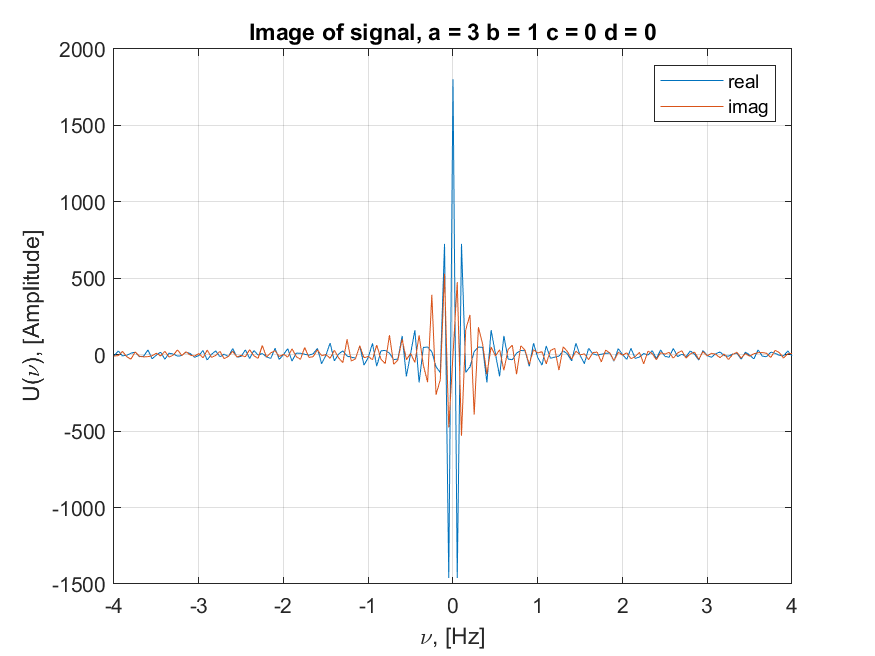
\includegraphics[width=0.8\textwidth]{image_a=3_b=1_c=0_d=0.png}
    \caption{Фурье-образ зашумлённого сигнала}
\end{figure}

\begin{figure}[ht]
    \centering
    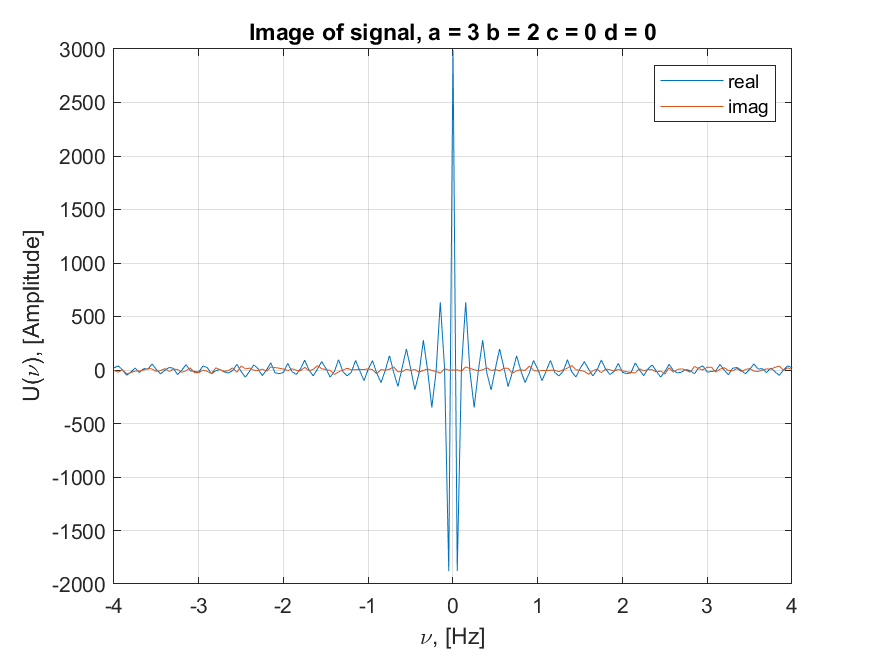
\includegraphics[width=0.8\textwidth]{image_a=3_b=2_c=0_d=0.png}
    \caption{Фурье-образ зашумлённого сигнала}
\end{figure}

\begin{figure}[ht]
    \centering
    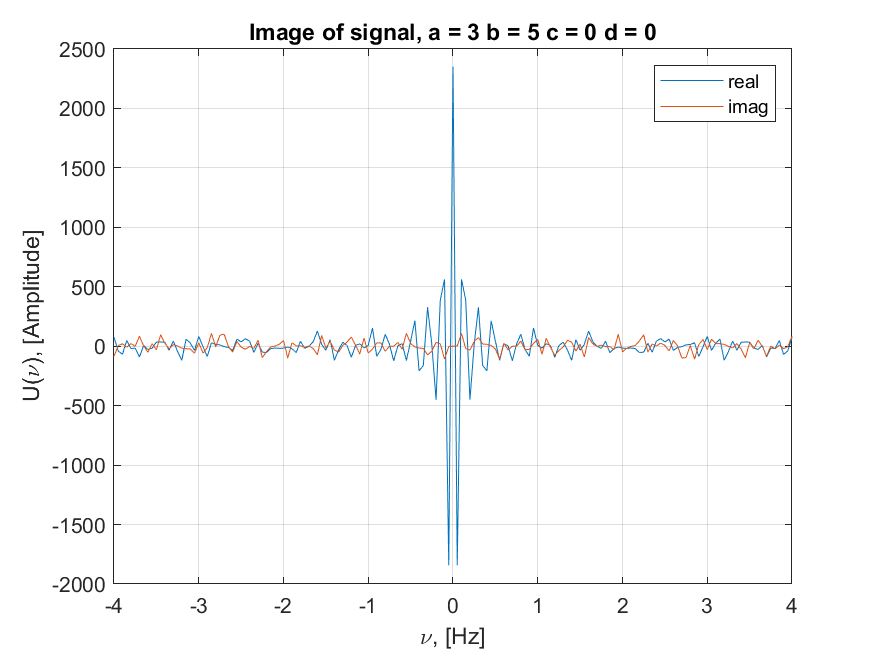
\includegraphics[width=0.8\textwidth]{image_a=3_b=5_c=0_d=0.png}
    \caption{Фурье-образ зашумлённого сигнала}
\end{figure}

\begin{figure}[ht]
    \centering
    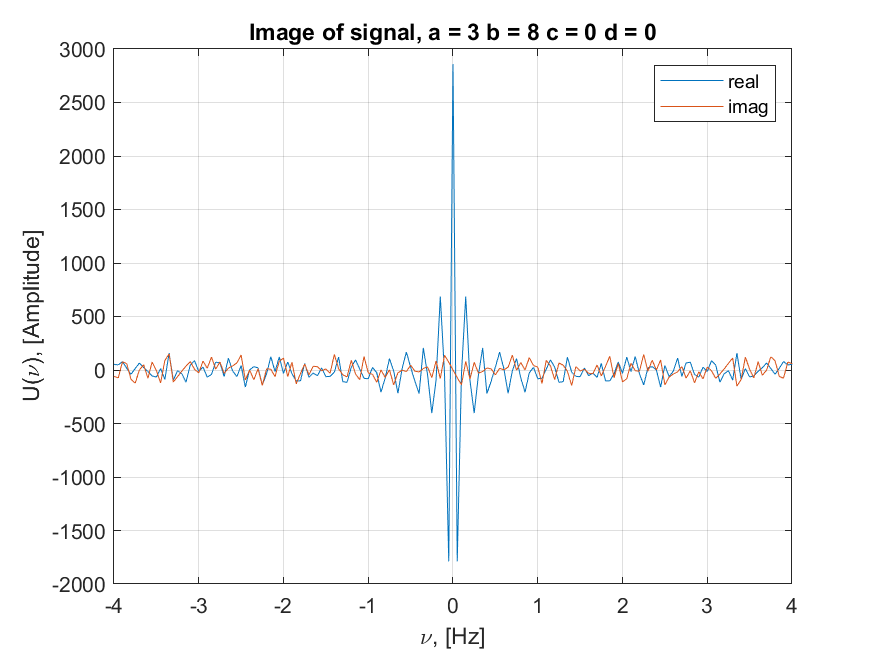
\includegraphics[width=0.8\textwidth]{image_a=3_b=8_c=0_d=0.png}
    \caption{Фурье-образ зашумлённого сигнала}
\end{figure}

\newpage
\subsection{Применяем фильтр}
В нашем случае ступенька фильтра будет около середины, потому что мы сохраняем нижние частоты, а они сосредоточены около начала графика. Будем применять разные диапазоны фильтра:

\begin{figure}[ht]
    \centering
    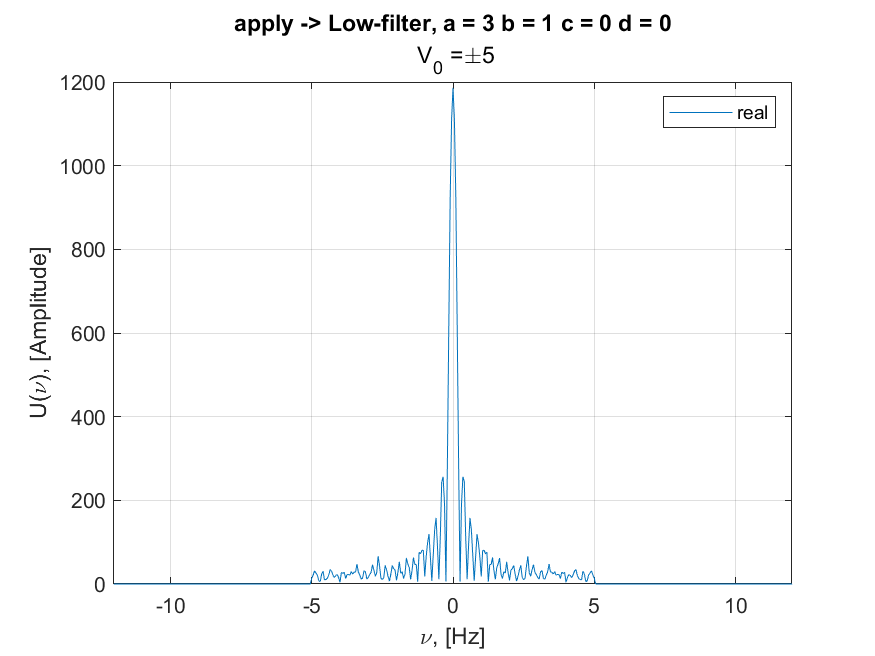
\includegraphics[width=0.8\textwidth]{applied_filter_a=3_b=1_c=0_d=0.png}
    \caption{Применили фильтр нижних частот}
\end{figure}

\begin{figure}[ht]
    \centering
    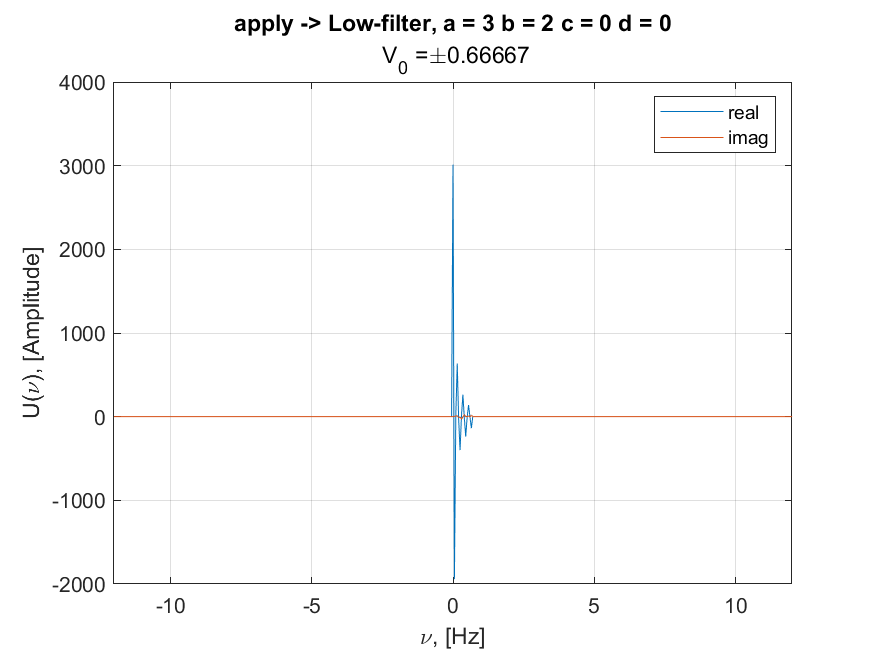
\includegraphics[width=0.8\textwidth]{applied_filter_a=3_b=2_c=0_d=0.png}
    \caption{Применили фильтр нижних частот}
\end{figure}

\begin{figure}[ht]
    \centering
    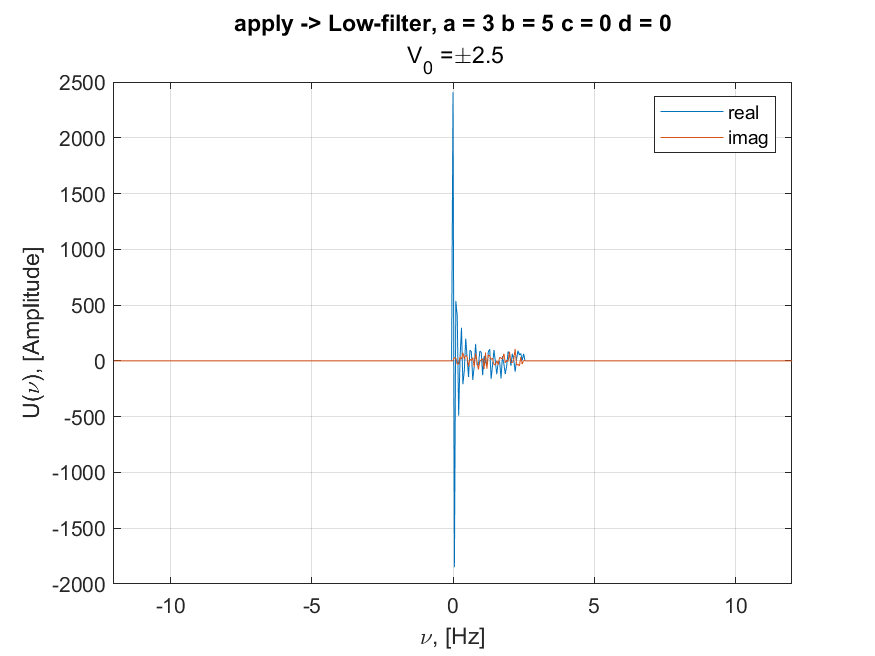
\includegraphics[width=0.8\textwidth]{applied_filter_a=3_b=5_c=0_d=0.png}
    \caption{Применили фильтр нижних частот}
\end{figure}

\begin{figure}[ht]
    \centering
    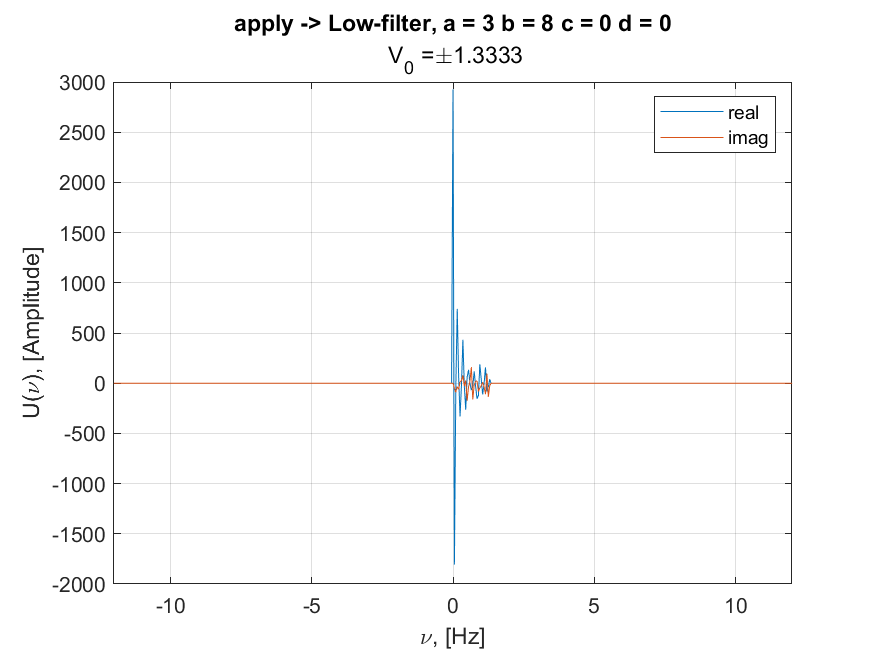
\includegraphics[width=0.8\textwidth]{applied_filter_a=3_b=8_c=0_d=0.png}
    \caption{Применили фильтр нижних частот}
\end{figure}

\newpage
\subsection{Возвращаемся к очищенному сигналу}

\begin{figure}[ht]
    \centering
    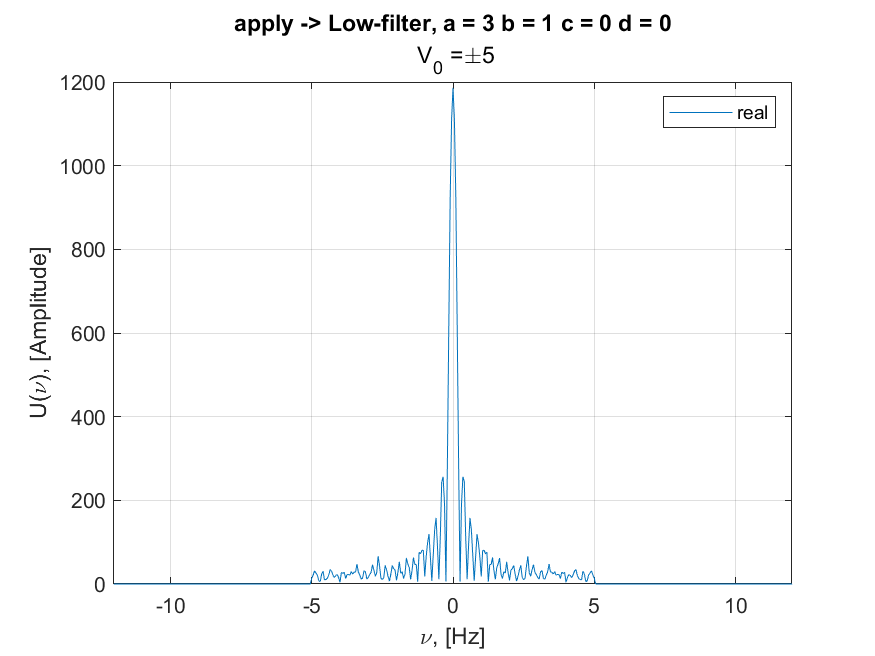
\includegraphics[width=0.8\textwidth]{applied_filter_a=3_b=1_c=0_d=0.png}
    \caption{Применили обратное преобразование Фурье}
\end{figure}

\begin{figure}[ht]
    \centering
    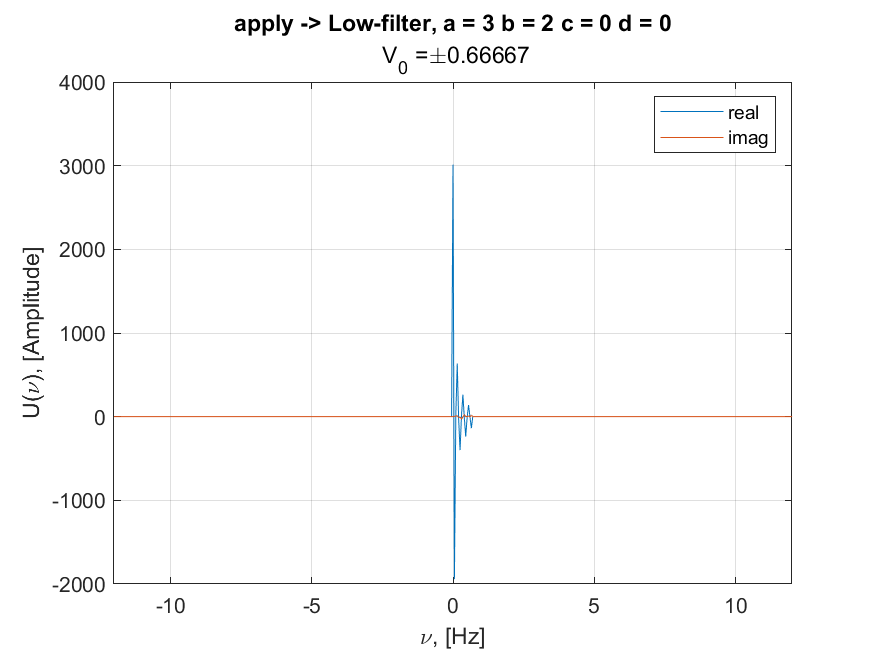
\includegraphics[width=0.8\textwidth]{applied_filter_a=3_b=2_c=0_d=0.png}
    \caption{Применили обратное преобразование Фурье}
\end{figure}

\begin{figure}[ht]
    \centering
    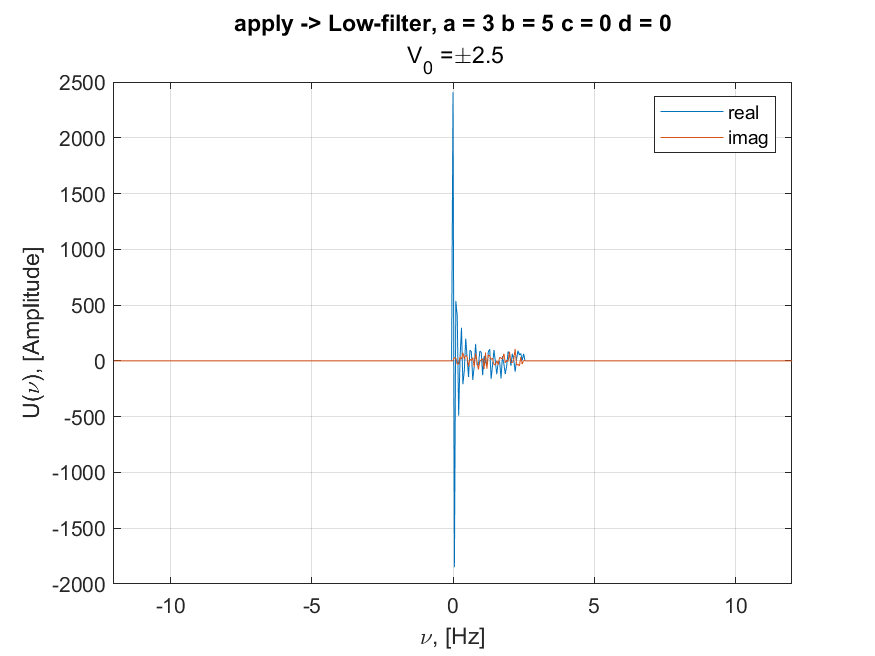
\includegraphics[width=0.8\textwidth]{applied_filter_a=3_b=5_c=0_d=0.png}
    \caption{Применили обратное преобразование Фурье}
\end{figure}

\begin{figure}[ht]
    \centering
    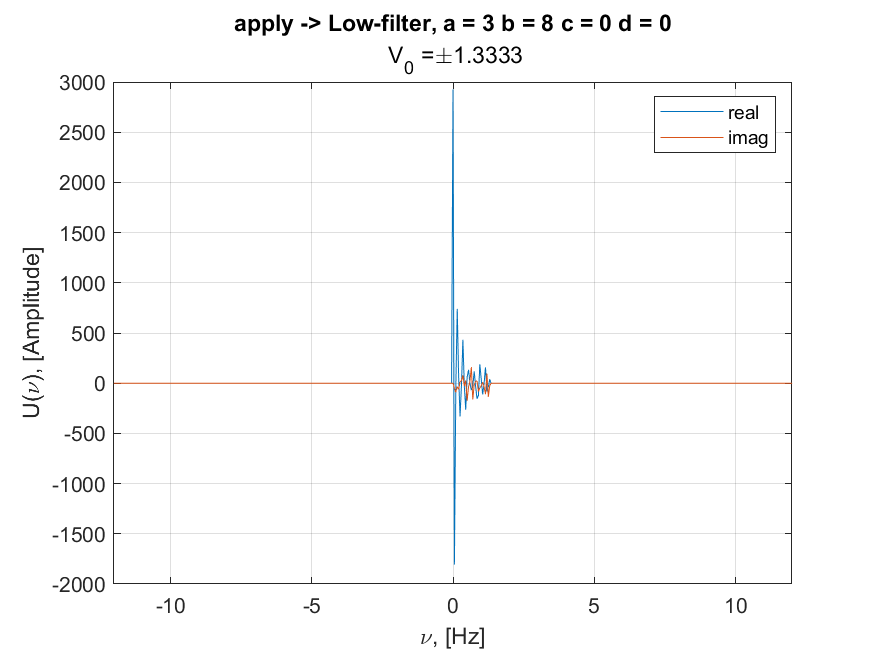
\includegraphics[width=0.8\textwidth]{applied_filter_a=3_b=8_c=0_d=0.png}
    \caption{Применили обратное преобразование Фурье}
\end{figure}

\subsection{Выводы}

Оставьте его неизменным для некоторого диапазона частот $[−\nu_0, \nu_0]$, но обнулите
его значения на всех остальных частотах, после чего выполните обратное преобразование Фурье. Постройте сравнительные графики исходного и фильтрованного
сигналов (для большей наглядности имеет смысл выводить на график лишь некоторую окрестность интервала [t1, t2]). Постройте сравнительные графики модуля
Фурье-образа исходного и фильтрованного сигналов. Исследуйте влияние частоты
среза ν0 и значения параметра b на эффективность фильтрации.


\section{Убираем специфические частоты}

Выберем все параметры $b, c, d$ ненулевыми. Теперь мы уже имеем дело с двумя компонентами шума - случайным и гармоническим. Соответственно, чтобы убрать обе компоненты, надо применить два фильтра, один из них мы уже нашли в пункте до.

\subsection{Фурье-образ сигнала u}

\subsection{Применяем фильтр}
Постараемся обнулить Фурье-образ на некоторых диапазонах частот, чтобы максимально убрать влияние обеих компонент помехи\dots

\subsection{Возвращаемся к очищенному сигналу}
Постройте сравнительные графики исходного и фильтрованного сигналов, а также графики модулей их Фурье образов. Исследуйте влияние частот среза, а также значений параметров b, c, d
на вид помехи и эффективность фильтрации (отдельно рассмотрите случай b=0).

\subsection{Выводы}



\section{Убираем низкие частоты?}

Рассмотрите фильтр, который обнуляет Фурье-образ
на всех частотах в некоторой окрестности точки ν = 0. Пропустите сигнал через
такой фильтр и оцените результат. Сделайте выводы.



% \begin{figure}[ht]
%     \centering
%     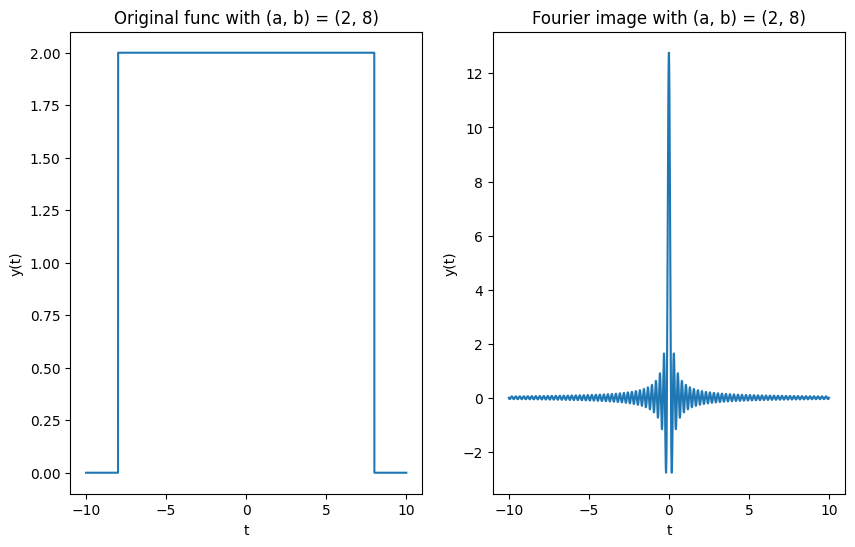
\includegraphics[width=0.9\textwidth]{f1_1.png}
%     \caption{График и образ прямоугольной функции}
% \end{figure}


\endinput